\documentclass{article}
\usepackage{graphicx}
\usepackage{subfigure}
\usepackage{dcolumn}
\usepackage{epstopdf}
\usepackage{textcomp}
\usepackage{float}
\usepackage{cite}
\usepackage{enumerate}
\usepackage{amssymb}
\usepackage{fancyhdr}
\usepackage{pdfpages}

\renewcommand{\rmdefault}{phv} % Arial
\renewcommand{\sfdefault}{phv} % Arial

\title{Software Development Process Report of \\ Group Project D}
\author{Group 34\\Kaixuan. Fan 1612313\\Tianyu. Zhang 1611800\\Qifan. Yan 1611277\\Minxing. Zhang 1612117}
\date{June 03, 2018}

\begin{document}
\maketitle

\newpage
\tableofcontents

\newpage
\pagestyle{fancy}
\lhead{\bfseries June 03, 2018\\ }
\chead{}
\rhead{\bfseries Software Development Process Report of \\ Group Project D}

\section{Problem Statement}
In this project, team members are required to develop a management system for a restaurant with the C++ programming language. The specific requirements for this management system are listed below:
\begin{enumerate}
    \item Above all, this management system must be capable of storing information related to the materials, dishes, menu, customers, orders, chefs and managers.
    \item This system should enable users to log in or sign up their personal accounts with specific passwords. After logging in or signing up, this system shold automatically distinguish the identity of the user (customer, chef or manager) and enter the appropriate interface.
    \item For different users (customer, chef or manager), this system should provide different functions. Different users are set to have different levels of access to these functions.
    \begin{itemize}
        \item For customers:\newline Customers should be able to browse the menu, create and modify the order, checkout. This system should calculate the total cost of a customer according to his or her order form. In addition, customers can edit their account information and log out their accounts.
        \item For chefs:\newline Chefs should be able to search and browse the information of raw materials and edit the menu. In addition, chefs can edit their account information and log out their accounts.
        \item For managers: \newline Managers have the highest authority to perform all the functions. Managers should be able to browse the information of customers, chefs and managers, add or delete them, and change the passwords of their accounts. Similarly, managers can also browse the information of the menu, materials and orders and edit them. In addition, managers can edit their account information and log out their accounts.
    \end{itemize}
    \item Finally, this system should calculate the gross profit according to the price of the materials and the cost of customers' order form.
\end{enumerate}







\section{Analysis}






\section{Design}







\section{Implementation}






\section{Testing}
\subsection{Tests for the logging in and signing up process}
\subsubsection{Logging in process}
\begin{enumerate}
    \item Check and prevent the invalid inputs. 
        \begin{figure}[H]
        \centering
        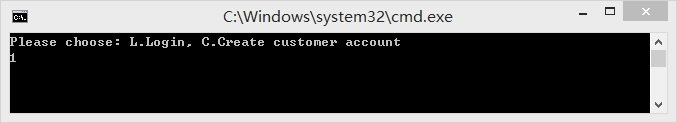
\includegraphics[width=0.85\textwidth]{login/00.jpg}
        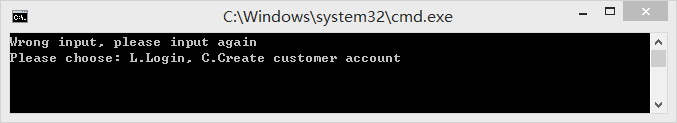
\includegraphics[width=0.85\textwidth]{login/01.jpg}
        \caption{Invalid inputs}
        \end{figure}
    \item Check and prevent the unregistered users.
        \begin{figure}[H]
        \centering
        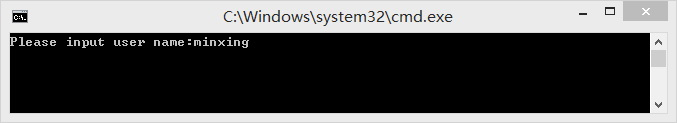
\includegraphics[width=0.85\textwidth]{login/21a.jpg}
        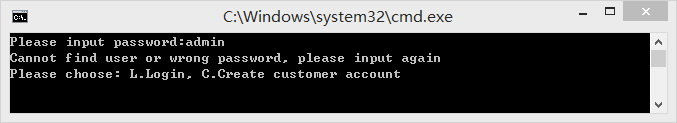
\includegraphics[width=0.85\textwidth]{login/21c.jpg}
        \caption{Unregistered users}
        \end{figure}
    \item Check and prevent the wrong passwords.
        \begin{figure}[H]
        \centering
        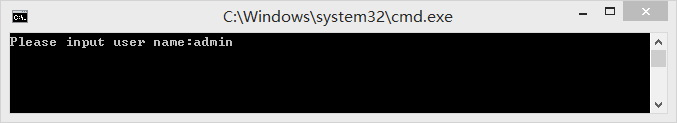
\includegraphics[width=0.85\textwidth]{login/22a.jpg}
        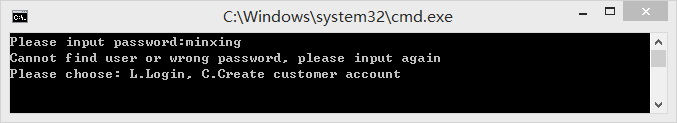
\includegraphics[width=0.85\textwidth]{login/22c.jpg}
        \caption{Wrong passwords}
        \end{figure}
    \item Successful login.
        \begin{figure}[H]
        \centering
        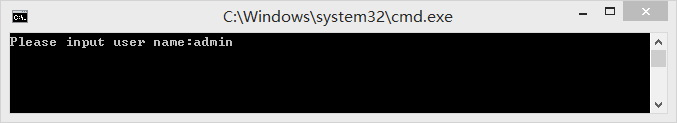
\includegraphics[width=0.85\textwidth]{login/23a.jpg}
        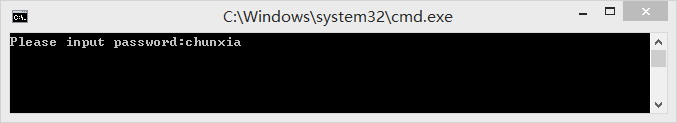
\includegraphics[width=0.85\textwidth]{login/23b.jpg}
        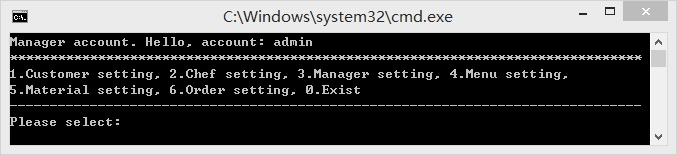
\includegraphics[width=0.85\textwidth]{login/23c.jpg}
        \caption{Successful login}
        \end{figure}
\end{enumerate}


\subsubsection{Signing up process}
\begin{enumerate}
    \item The username of different accounts are not allowed to be duplicated.
        \begin{figure}[H]
        \centering
        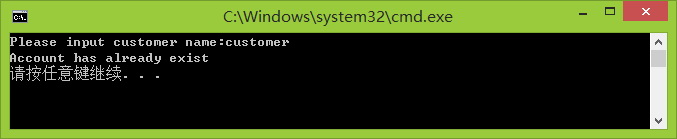
\includegraphics[width=0.85\textwidth]{signup/10.jpg}
        \caption{Duplicate username}
        \end{figure}
    \item Set an available username and password to create a customer account.
        \begin{figure}[H]
        \centering
        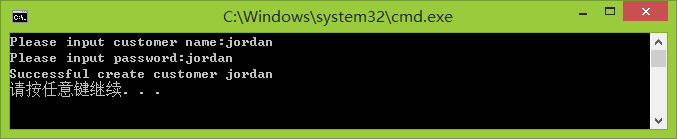
\includegraphics[width=0.85\textwidth]{signup/11.jpg}
        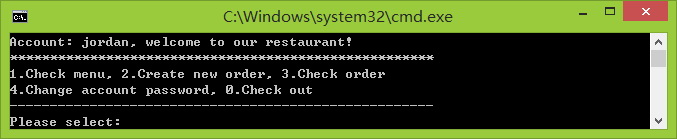
\includegraphics[width=0.85\textwidth]{signup/12.jpg}
        \caption{Customer account}
        \end{figure}
\end{enumerate}






\subsection{Tests for the functions of manager accounts}
After the manager logging in successfully, the initial interface of the manager account is shown below:
\begin{figure}[H]
    \centering
    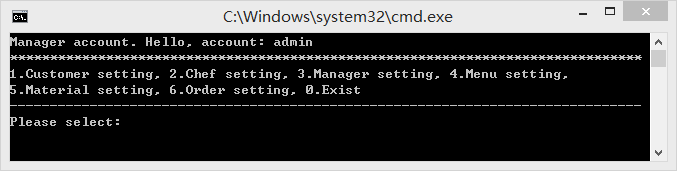
\includegraphics[width=0.85\textwidth]{manager0000.png}
    \caption{Initial interface}
\end{figure}


\subsubsection{Set customer}
When the manager enters 1, the system will enter the interface for setting customers.
\begin{figure}[H]
    \centering
    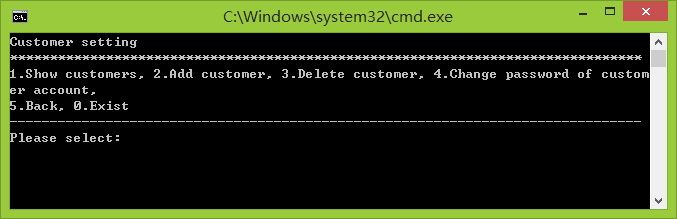
\includegraphics[width=0.85\textwidth]{A/02.jpg}
    \caption{Interface for setting customers.}
\end{figure}

\begin{enumerate}
    \item Show customer:\newline 
    When the manager enters 1, the system will display the customer list.
        \begin{figure}[H]
        \centering
        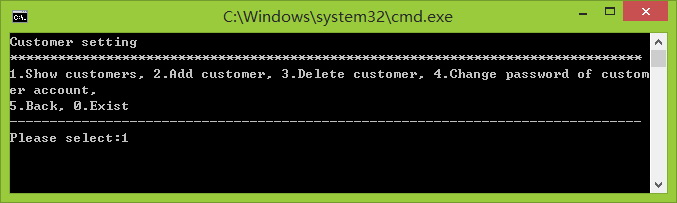
\includegraphics[width=0.85\textwidth]{A/A1a.jpg}
        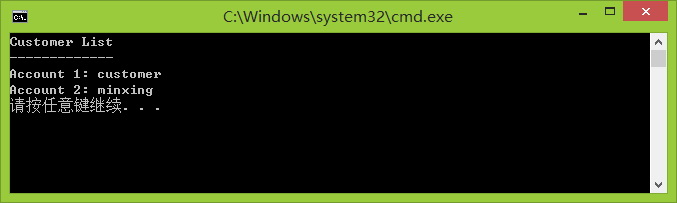
\includegraphics[width=0.85\textwidth]{A/A1b.jpg}
        \caption{Customer list}
        \end{figure}
    
    \item Add customer:\newline 
    When the manager enters 2, the system will enter the program for creating a customer account.
        \begin{figure}[H]
        \centering
        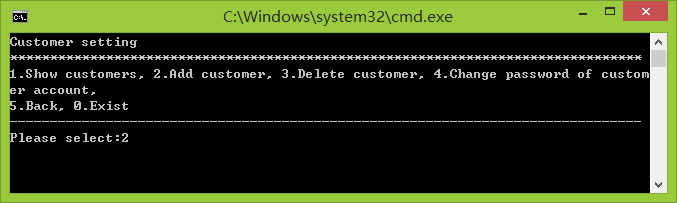
\includegraphics[width=0.85\textwidth]{A/A2a.jpg}
        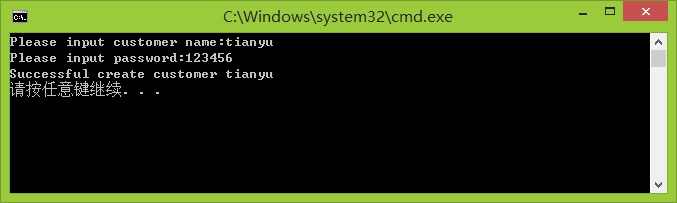
\includegraphics[width=0.85\textwidth]{A/A2b.jpg}
        \caption{Create a customer account}
        \end{figure}
    \noindent
    If the username of the customer account is founded to be duplicated, the program will prompt to re-enter and return to the previous interface.
        \begin{figure}[H]
        \centering
        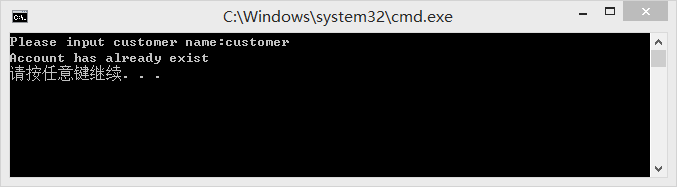
\includegraphics[width=0.85\textwidth]{A/A2c.png}
        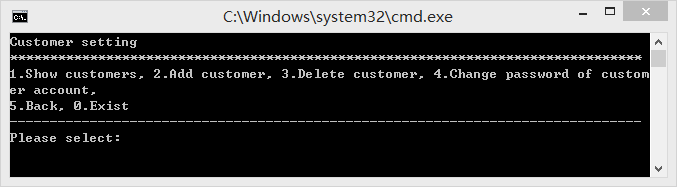
\includegraphics[width=0.85\textwidth]{A/A2d.png}
        \caption{Duplicate username}
        \end{figure}
    
    \item Delete customer:\newline 
    When the manager enters 3, the manager must enter the administrator password again, then the system will enter the program for deleting a customer account. 
        \begin{figure}[H]
        \centering
        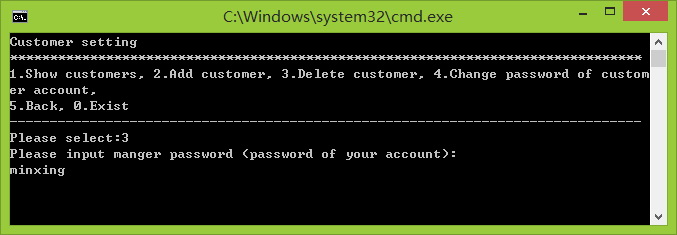
\includegraphics[width=0.85\textwidth]{A/A3a0.jpg}
        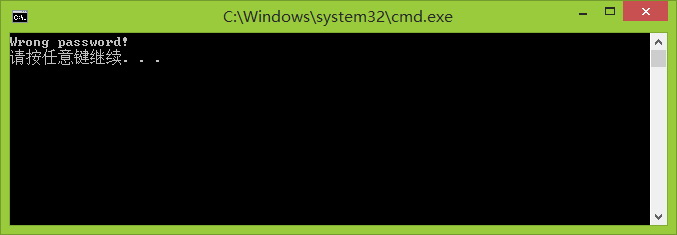
\includegraphics[width=0.85\textwidth]{A/A3a1.jpg}
        \caption{Wrong administrator password}
        \end{figure}
    \noindent
    Only when the manager enters the right administrator password, the program will allow the manager to delete a customer account. In addition, the program will automatically detect whether the entered username exists or not.
        \begin{figure}[H]
        \centering
        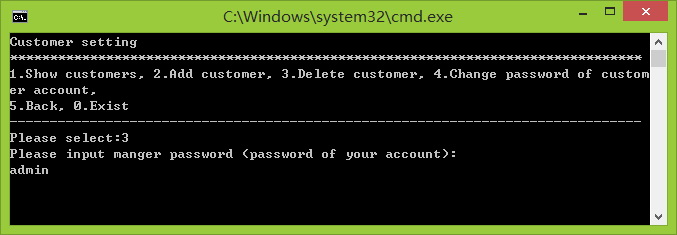
\includegraphics[width=0.85\textwidth]{A/A3b0.jpg}
        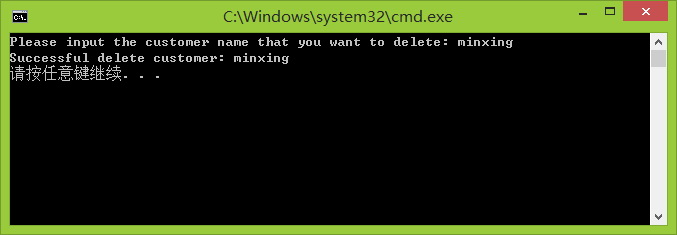
\includegraphics[width=0.85\textwidth]{A/A3b1.jpg}
        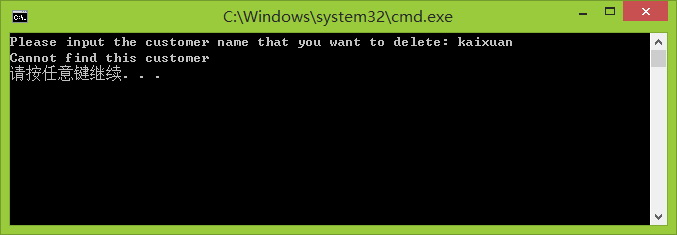
\includegraphics[width=0.85\textwidth]{A/A3b2.jpg}
        \caption{Delete customer}
        \end{figure}
    
    \item Set password of customer accounts:\newline 
    When the manager enters 4, only when the manager enters the right administrator password, the system will enter the program for setting the password of customer accounts. Similarly, the program will automatically detect whether the entered username exists or not.
        \begin{figure}[H]
        \centering
        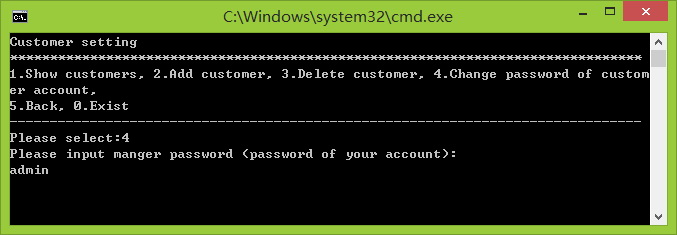
\includegraphics[width=0.85\textwidth]{A/A4b0.jpg}
        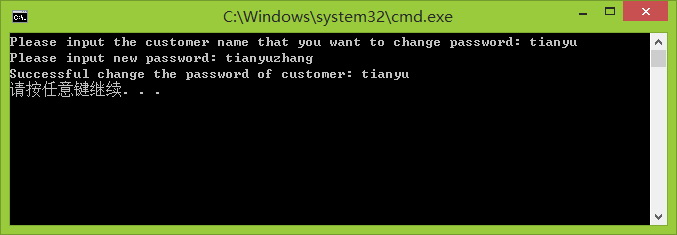
\includegraphics[width=0.85\textwidth]{A/A4b1.jpg}
        \caption{Set password of customer accounts}
        \end{figure}
    
    \item Back:\newline 
    When the manager enters 5, the system will return to the previous interface.
        \begin{figure}[H]
        \centering
        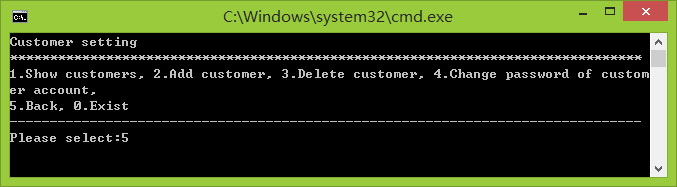
\includegraphics[width=0.85\textwidth]{A/A5a.jpg}
        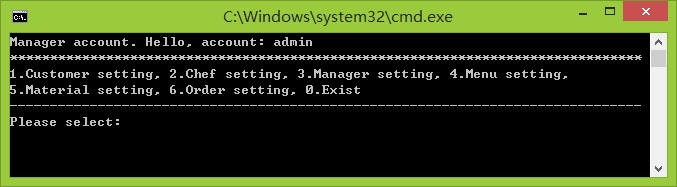
\includegraphics[width=0.85\textwidth]{A/A5b.jpg}
        \caption{Return to the previous interface}
        \end{figure}
    
    \item Log out:\newline
    When the manager enters 0, the manager will log out.
        \begin{figure}[H]
        \centering
        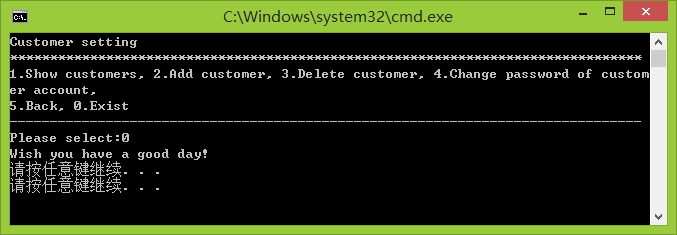
\includegraphics[width=0.85\textwidth]{A/A0.jpg}
        \caption{Log out}
        \end{figure}
    
\end{enumerate}


\subsubsection{Set chef}
When the manager enters 2, the system will enter the interface for setting chefs.
\begin{figure}[H]
    \centering
    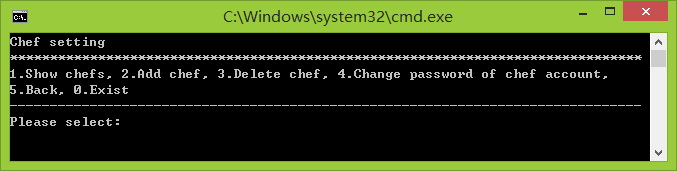
\includegraphics[width=0.85\textwidth]{B/02.jpg}
    \caption{Interface for setting chefs}
\end{figure}

\begin{enumerate}
    \item Show chef:\newline 
    When the manager enters 1, the system will display the chef list.
        \begin{figure}[H]
        \centering
        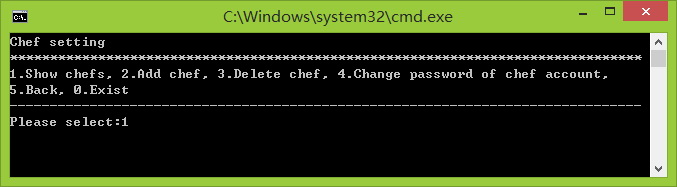
\includegraphics[width=0.85\textwidth]{B/B1a.jpg}
        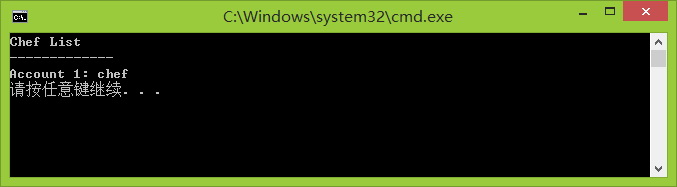
\includegraphics[width=0.85\textwidth]{B/B1b.jpg}
        \caption{Chef list}
        \end{figure}
    
    \item Add chef:\newline 
    When the manager enters 2, only when the manager enters the right administrator password, the system will enter the program for creating a chef account.
        \begin{figure}[H]
        \centering
        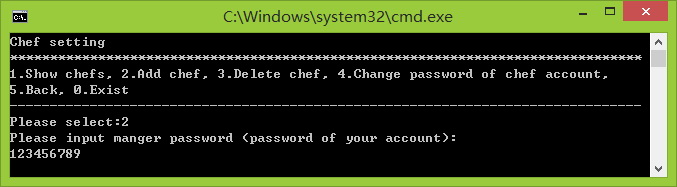
\includegraphics[width=0.85\textwidth]{B/B2a1.jpg}
        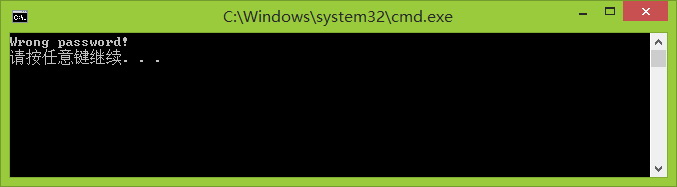
\includegraphics[width=0.85\textwidth]{B/B2a2.jpg}
        \caption{Wrong administrator password}
        \end{figure}
    \noindent
    If the username of the chef account is founded to be duplicated, the program will prompt to re-enter and return to the previous interface.
        \begin{figure}[H]
        \centering
        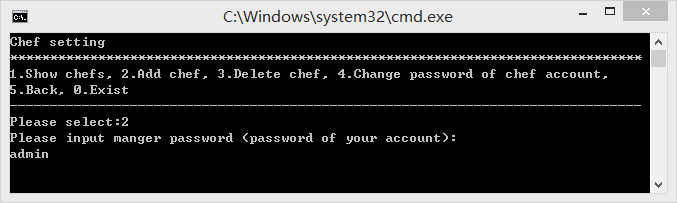
\includegraphics[width=0.85\textwidth]{B/B2c1.png}
        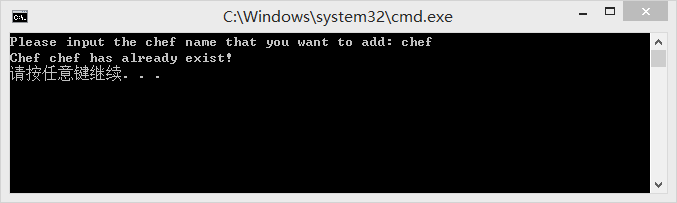
\includegraphics[width=0.85\textwidth]{B/B2c2.png}
        \caption{Duplicate username}
        \end{figure}
        \begin{figure}[H]
        \centering
        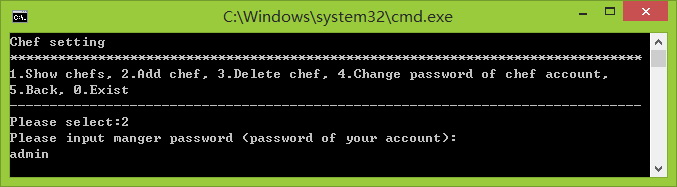
\includegraphics[width=0.85\textwidth]{B/B2b1.jpg}
        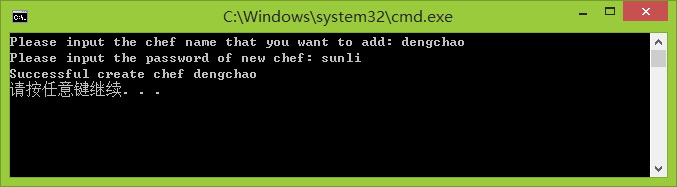
\includegraphics[width=0.85\textwidth]{B/B2b2.jpg}
        \caption{Create a chef account}
        \end{figure}
        
    \item Delete chef:\newline 
    When the manager enters 3, only when the manager enters the right administrator password, the system will enter the program for deleting a chef account. Similarly, the program will automatically detect whether the entered username exists or not.
        \begin{figure}[H]
        \centering
        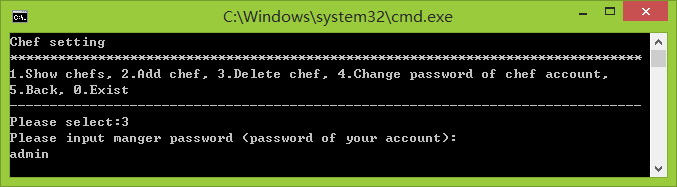
\includegraphics[width=0.85\textwidth]{B/B3b1.jpg}
        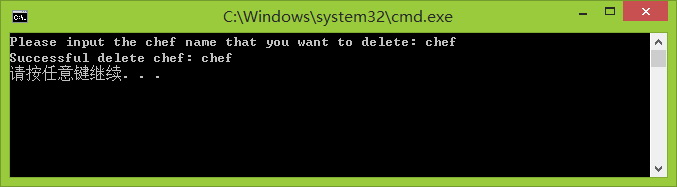
\includegraphics[width=0.85\textwidth]{B/B3b3.jpg}
        \caption{Delete chef}
        \end{figure}
    
    \item Set password of chef accounts:\newline 
    When the manager enters 4, only when the manager enters the right administrator password, the system will enter the program for setting the password of chef accounts. Similarly, the program will automatically detect whether the entered username exists or not.
        \begin{figure}[H]
        \centering
        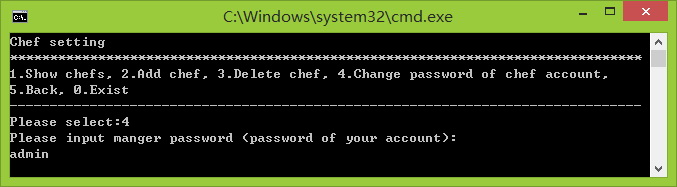
\includegraphics[width=0.85\textwidth]{B/B4b1.jpg}
        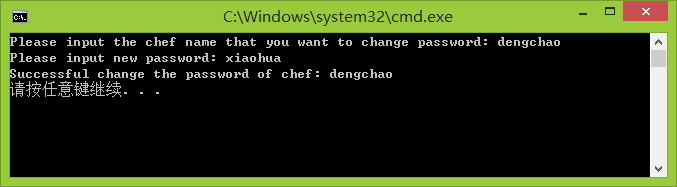
\includegraphics[width=0.85\textwidth]{B/B4b3.jpg}
        \caption{Set password of chef accounts}
        \end{figure}
    
    \item Back:\newline 
    When the manager enters 5, the system will return to the previous interface.
        \begin{figure}[H]
        \centering
        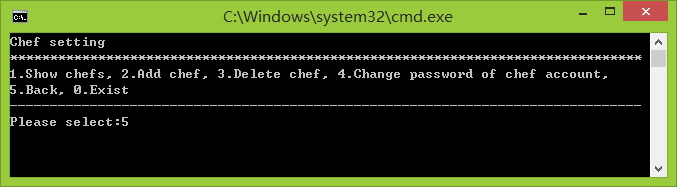
\includegraphics[width=0.85\textwidth]{B/B5a.jpg}
        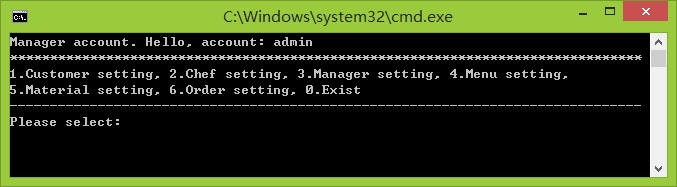
\includegraphics[width=0.85\textwidth]{B/B5b.jpg}
        \caption{Return to the previous interface}
        \end{figure}
    
    \item Log out:\newline
    When the manager enters 0, the manager will log out.
        \begin{figure}[H]
        \centering
        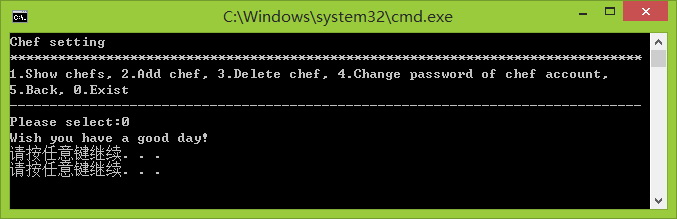
\includegraphics[width=0.85\textwidth]{B/B0.jpg}
        \caption{Log out}
        \end{figure}
    
\end{enumerate}


\subsubsection{Set manager}
When the manager enters 3, the system will enter the interface for setting managers.
\begin{figure}[H]
    \centering
    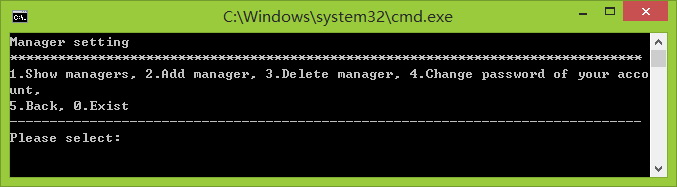
\includegraphics[width=0.85\textwidth]{C/02.jpg}
    \caption{Interface for setting managers}
\end{figure}

\begin{enumerate}
    \item Show manager:\newline 
    When the manager enters 1, only when the manager enters the right administrator password, the system will display the manager list.
        \begin{figure}[H]
        \centering
        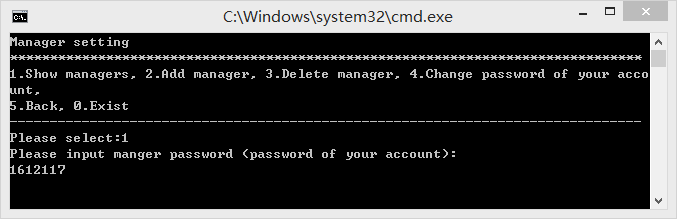
\includegraphics[width=0.85\textwidth]{C/222222a.png}
        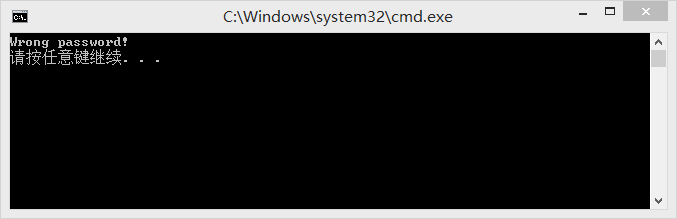
\includegraphics[width=0.85\textwidth]{C/222222b.png}
        \caption{Wrong administrator password}
        \end{figure}
        \begin{figure}[H]
        \centering
        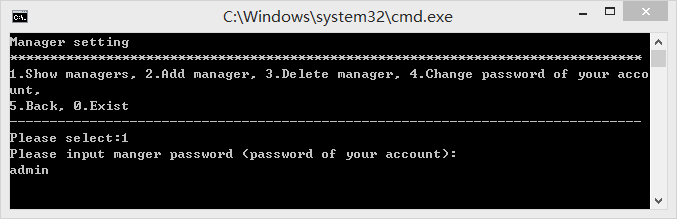
\includegraphics[width=0.85\textwidth]{C/222222c.png}
        \includegraphics[width=0.85\textwidth]{C/222222d.png}
        \caption{Manager list}
        \end{figure}
    
    \item Add manager:\newline 
    When the manager enters 2, similarly, only when the manager enters the right administrator password, the system will enter the program for creating a manager account. In addition, if the username of the manager account is founded to be duplicated, the program will prompt to re-enter and return to the previous interface.
        \begin{figure}[H]
        \centering
        \includegraphics[width=0.85\textwidth]{C/222233b.png}
        \includegraphics[width=0.85\textwidth]{C/222233d.png}
        \caption{Duplicate username}
        \end{figure}
        \begin{figure}[H]
        \centering
        \includegraphics[width=0.85\textwidth]{C/222233a.png}
        \includegraphics[width=0.85\textwidth]{C/222233c.png}
        \caption{Create a manager account}
        \end{figure}
        
    \item Delete manager:\newline 
    When the manager enters 3, only when the manager enters the right administrator password, the system will enter the program for deleting a manager account. Similarly, the program will automatically detect whether the entered username exists or not.
        \begin{figure}[H]
        \centering
        \includegraphics[width=0.85\textwidth]{C/C3b1.jpg}
        \includegraphics[width=0.85\textwidth]{C/C3b3.jpg}
        \includegraphics[width=0.85\textwidth]{C/C3b2.jpg}
        \caption{Delete manager}
        \end{figure}
    
    \item Set password of manager accounts:\newline 
    When the manager enters 4, only when the manager enters the right administrator password, the system will enter the program for setting the new password of current manager account. 
        \begin{figure}[H]
        \centering
        \includegraphics[width=0.85\textwidth]{C/C4b1.jpg}
        \includegraphics[width=0.85\textwidth]{C/C4b2.jpg}
        \caption{Set password of manager accounts}
        \end{figure}
    
    \item Back:\newline 
    When the manager enters 5, the system will return to the previous interface.
        \begin{figure}[H]
        \centering
        \includegraphics[width=0.85\textwidth]{C/C5a.jpg}
        \includegraphics[width=0.85\textwidth]{C/C5b.jpg}
        \caption{Return to the previous interface}
        \end{figure}
    
    \item Log out:\newline
    When the manager enters 0, the manager will log out.
        \begin{figure}[H]
        \centering
        \includegraphics[width=0.85\textwidth]{C/C0.jpg}
        \caption{Log out}
        \end{figure}
    
\end{enumerate}


\subsubsection{Set menu}
When the manager enters 4, the system will enter the interface for setting menu.
\begin{figure}[H]
    \centering
    \includegraphics[width=0.85\textwidth]{D/02.jpg}
    \caption{Interface for setting menu}
\end{figure}

\begin{enumerate}
    \item Show menu:\newline 
    When the manager enters 1, the system will display the menu of the restaurant.
        \begin{figure}[H]
        \centering
        \includegraphics[width=0.85\textwidth]{D/D1a.jpg}
        \includegraphics[width=0.85\textwidth]{D/D11111111.png}
        \caption{Menu}
        \end{figure}
    
    \item Add dishes:\newline 
    When the manager enters 2, the system will enter the program for adding dishes.
        \begin{figure}[H]
        \centering
        \includegraphics[width=0.85\textwidth]{D/D2a.jpg}
        \includegraphics[width=0.85\textwidth]{D/D2b.jpg}
        \caption{Add dishes}
        \end{figure}
    \noindent
    If the ID or name of new dishes are founded to be duplicated, the program will prompt to re-enter.
        \begin{figure}[H]
        \centering
        \includegraphics[width=0.85\textwidth]{D/D2c.jpg}
        \caption{Duplicate ID or name}
        \end{figure}
    \noindent
    Then, the program will require the manager to select materials for the dishes from the material list. The program will automatically detect whether the materials selected by the manager are on the material list or not. If not, the program will prompt the manager to re-select. In addition, the program will ask the manager if he or she would like to add other materials every time the manager select a material.
        \begin{figure}[H]
        \centering
        \includegraphics[width=0.8\textwidth]{D/D222221.png}
        \includegraphics[width=0.8\textwidth]{D/D222221.png}
        \caption{Select materials for dishes}
        \end{figure}
    
    \item Set dishes:\newline 
    When the manager enters 3, the system will enter the program for setting dishes.
        \begin{figure}[H]
        \centering
        \includegraphics[width=0.8\textwidth]{D/D3a.jpg}
        \includegraphics[width=0.8\textwidth]{D/D3c1.jpg}
        \includegraphics[width=0.8\textwidth]{D/D3c2.jpg}
        \caption{Select a dish to modify}
        \end{figure}
        
    \item Delete dishes:\newline 
    When the manager enters 4, the system will enter the program for deleting dishes. 
        \begin{figure}[H]
        \centering
        \includegraphics[width=0.8\textwidth]{D/D4a1.jpg}
        \includegraphics[width=0.8\textwidth]{D/D4c1.jpg}
        \caption{Delete dishes}
        \end{figure}
    
    \item Back:\newline 
    When the manager enters 5, the system will return to the previous interface.
        \begin{figure}[H]
        \centering
        \includegraphics[width=0.85\textwidth]{D/D5a.jpg}
        \includegraphics[width=0.85\textwidth]{D/D5b.jpg}
        \caption{Return to the previous interface}
        \end{figure}
    
    \item Log out:\newline
    When the manager enters 0, the manager will log out.
        \begin{figure}[H]
        \centering
        \includegraphics[width=0.85\textwidth]{D/D0.jpg}
        \caption{Log out}
        \end{figure}
    
\end{enumerate}


\subsubsection{Set material}
When the manager enters 5, the system will enter the interface for setting materials.
\begin{figure}[H]
    \centering
    \includegraphics[width=0.85\textwidth]{E/02.jpg}
    \caption{Interface for setting materials}
\end{figure}

\begin{enumerate}
    \item Show material:\newline 
    When the manager enters 1, the system will display the material list.
        \begin{figure}[H]
        \centering
        \includegraphics[width=0.85\textwidth]{E/E1a.jpg}
        \includegraphics[width=0.85\textwidth]{E/E1b.jpg}
        \caption{Material list}
        \end{figure}
    
    \item Add material:\newline 
    When the manager enters 2, the system will enter the program for adding materials. The program will automatically detect whether the ID of this new material has been occupied by other materials.
        \begin{figure}[H]
        \centering
        \includegraphics[width=0.85\textwidth]{E/E2a.jpg}
        \includegraphics[width=0.85\textwidth]{E/E2b.jpg}
        \caption{Add material}
        \end{figure}
    
    \item Set material:\newline 
    When the manager enters 4, the system will enter the program for setting materials. 
        \begin{figure}[H]
        \centering
        \includegraphics[width=0.85\textwidth]{E/E3a.jpg}
        \includegraphics[width=0.85\textwidth]{E/E3allin.jpg}
        \caption{Set materials}
        \end{figure}
    
    \item Delete material:\newline 
    When the manager enters 4, the system will enter the program for deleting materials. 
        \begin{figure}[H]
        \centering
        \includegraphics[width=0.85\textwidth]{E/E4a.jpg}
        \includegraphics[width=0.85\textwidth]{E/E4b0.jpg}
        \caption{Enter ID}
        \end{figure}
        \begin{figure}[H]
        \centering
        \includegraphics[width=0.8\textwidth]{E/E4b1b.jpg}
        \includegraphics[width=0.8\textwidth]{E/E4b1a.jpg}
        \caption{Delete material (Yes or No)}
        \end{figure}
        
    \item Back:\newline 
    When the manager enters 5, the system will return to the previous interface.
        \begin{figure}[H]
        \centering
        \includegraphics[width=0.85\textwidth]{E/E5a.jpg}
        \includegraphics[width=0.85\textwidth]{E/E5b.jpg}
        \caption{Return to the previous interface}
        \end{figure}
    
    \item Log out:\newline
    When the manager enters 0, the manager will log out.
        \begin{figure}[H]
        \centering
        \includegraphics[width=0.85\textwidth]{E/000000000.png}
        \caption{Log out}
        \end{figure}
    
\end{enumerate}


\subsubsection{Set order}
When the manager enters 6, the system will enter the interface for setting orders.
\begin{figure}[H]
    \centering
    \includegraphics[width=0.85\textwidth]{F/02.jpg}
    \caption{Interface for setting orders}
\end{figure}

\begin{enumerate}
    \item Show order:\newline 
    When the manager enters 1, the system will display the order list.
        \begin{figure}[H]
        \centering
        \includegraphics[width=0.85\textwidth]{F/F1a.jpg}
        \includegraphics[width=0.85\textwidth]{F/F1b.jpg}
        \caption{Order list}
        \end{figure}
    
    \item Add order:\newline
    When the manager enters 1, the system will enter the program for adding an order. 
        \begin{figure}[H]
        \centering
        \includegraphics[width=0.85\textwidth]{F/F222221.png}
        \includegraphics[width=0.85\textwidth]{F/F2c2.jpg}
        \caption{Process of adding an order}
        \end{figure}
        
    \item Delete order:\newline
    When the manager enters 1, the system will enter the program for deleting an order.
        \begin{figure}[H]
        \centering
        \includegraphics[width=0.85\textwidth]{F/F3a.jpg}
        \includegraphics[width=0.85\textwidth]{F/F3b1.jpg}
        \includegraphics[width=0.85\textwidth]{F/F3b2.jpg}
        \caption{Delete an order}
        \end{figure}
        
    \item Back:\newline 
    When the manager enters 4, the system will return to the previous interface.
        \begin{figure}[H]
        \centering
        \includegraphics[width=0.85\textwidth]{F/F4a.jpg}
        \includegraphics[width=0.85\textwidth]{F/F4b.jpg}
        \caption{Return to the previous interface}
        \end{figure}
    
    \item Log out:\newline 
    When the manager enters 0, the manager will log out.
        \begin{figure}[H]
        \centering
        \includegraphics[width=0.85\textwidth]{F/F0.jpg}
        \caption{Log out}
        \end{figure}
    
\end{enumerate}


\subsubsection{Log out}
When the manager enters 0, the manager will log out.
\begin{figure}[H]
    \centering
    \includegraphics[width=0.85\textwidth]{login/adminexit.jpg}
    \caption{Log out}
\end{figure}






\subsection{Tests for the functions of chef accounts}
After the chef logging in successfully, the initial interface of the chef account is shown below:
\begin{figure}[H]
    \centering
    \includegraphics[width=0.85\textwidth]{Q/00.jpg}
    \caption{Initial interface}
\end{figure}

\subsubsection{Set menu}
When the chef enters 2, the system will enter the interface for setting menu.
\begin{figure}[H]
    \centering
    \includegraphics[width=0.85\textwidth]{Q/1/Q_0b1.jpg}
    \caption{Interface for setting menu}
\end{figure}
        
\begin{enumerate}
    \item Show menu:\newline 
    When the chef enters 1, the system will display the menu of the restaurant.
        \begin{figure}[H]
        \centering
        \includegraphics[width=0.85\textwidth]{Q/1/Q_1a.jpg}
        \includegraphics[width=0.85\textwidth]{Q/1/Q_1b.jpg}
        \caption{Menu interface}
        \end{figure}
        
    \item Add dishes:\newline 
    When the chef enters 2, the system will enter the program for adding dishes.
        \begin{figure}[H]
        \centering
        \includegraphics[width=0.85\textwidth]{Q/1/Q_2a.jpg}
        \includegraphics[width=0.85\textwidth]{Q/1/222221.png}
        \caption{Add dishes}
        \end{figure}
        \begin{figure}[H]
        \centering
        \includegraphics[width=0.85\textwidth]{Q/1/222222.png}
        \includegraphics[width=0.85\textwidth]{Q/1/222223.png}
        \caption{Select materials for the dish}
        \end{figure}
        
    \item Set dishes:\newline 
    When the chef enters 3, the system will enter the interface for setting dishes.
        \begin{figure}[H]
        \centering
        \includegraphics[width=0.85\textwidth]{Q/1/Q_3a.jpg}
        \includegraphics[width=0.85\textwidth]{Q/1/333331.png}
        \caption{Select dishes}
        \end{figure}
        \begin{figure}[H]
        \centering
        \includegraphics[width=0.85\textwidth]{Q/1/333332.png}
        \includegraphics[width=0.85\textwidth]{Q/1/333333.png}
        \includegraphics[width=0.85\textwidth]{Q/1/333334.png}
        \includegraphics[width=0.85\textwidth]{Q/1/333335.png}
        \includegraphics[width=0.85\textwidth]{Q/1/333336.png}
        \includegraphics[width=0.85\textwidth]{Q/1/333337.png}
        \includegraphics[width=0.85\textwidth]{Q/1/333338.png}
        \caption{Set dishes}
        \end{figure}
        
    \item Delete dishes:\newline 
    When the chef enters 4, the program will enter the interface for deleting dishes. The program will automatically detect whether the dishes which the chef will delete exist or not.
        \begin{figure}[H]
        \centering
        \includegraphics[width=0.85\textwidth]{Q/1/444440.png}
        \includegraphics[width=0.85\textwidth]{Q/1/444443.png}
        \includegraphics[width=0.85\textwidth]{Q/1/444442.png}
        \includegraphics[width=0.85\textwidth]{Q/1/444441.png}
        \caption{Delete dishes}
        \end{figure}
    
    
    \item Back:\newline 
    When the chef enters 5, the system will return to the previous interface.
        \begin{figure}[H]
        \centering
        \includegraphics[width=0.85\textwidth]{Q/1/Q_5a.jpg}
        \includegraphics[width=0.85\textwidth]{Q/1/Q_5b.jpg}
        \caption{Return to the previous interface}
        \end{figure}
        
    \item Log out:\newline
    When the chef enters 0, the chef will log out.
        \begin{figure}[H]
        \centering
        \includegraphics[width=0.85\textwidth]{Q/1/Q_0.jpg}
        \caption{Log out}
        \end{figure}
        
\end{enumerate}


\subsubsection{Set material}
When the chef enters 1, the system will enter the interface for setting materials.
\begin{figure}[H]
    \centering
    \includegraphics[width=0.85\textwidth]{Q/2/Q_0b2.jpg}
    \caption{Interface for setting materials}
\end{figure}

\begin{enumerate}
    \item Show material:\newline 
    When the chef enters 1, the system will display the material interface.
        \begin{figure}[H]
        \centering
        \includegraphics[width=0.85\textwidth]{Q/2/Q_1a.jpg}
        \includegraphics[width=0.85\textwidth]{Q/2/Q_1b.jpg}
        \caption{Material list}
        \end{figure}
        
    \item Add material:\newline 
    When the chef enters 2, the system will enter the interface for adding materials.
        \begin{figure}[H]
        \centering
        \includegraphics[width=0.85\textwidth]{Q/2/222221.png}
        \includegraphics[width=0.85\textwidth]{Q/2/222222.png}
        \caption{Add materials}
        \end{figure}
        
    \item Set material:\newline 
    When the chef enters 3, the system will enter the interface for setting materials.
        \begin{figure}[H]
        \centering
        \includegraphics[width=0.85\textwidth]{Q/2/333331.png}
        \includegraphics[width=0.85\textwidth]{Q/2/333333.png}
        \caption{Set materials}
        \end{figure}
        
    \item Delete material:\newline 
    When the chef enters 4, the program will enter the interface for deleting materials.
        \begin{figure}[H]
        \centering
        \includegraphics[width=0.85\textwidth]{Q/2/444441.png}
        \includegraphics[width=0.85\textwidth]{Q/2/444442.png}
        \caption{Delete material}
        \end{figure}
        
    \item Back:\newline 
    When the chef enters 0, the system will return to the previous interface.
        \begin{figure}[H]
        \centering
        \includegraphics[width=0.85\textwidth]{Q/2/Q_5a.jpg}
        \includegraphics[width=0.85\textwidth]{Q/2/Q_5b.jpg}
        \caption{Return to the previous interface}
        \end{figure}
        
    \item Log out:\newline
    When the chef enters 0, the chef will log out.
        \begin{figure}[H]
        \centering
        \includegraphics[width=0.85\textwidth]{Q/2/Q_0.jpg}
        \caption{Log out}
        \end{figure}
        
\end{enumerate}



\subsubsection{Set password}
When the chef enters 4, the program will first prompt the chef to enter the previous password. When the previous password is wrong, the system will exit the password modification program. Only when the previous password is right, the system will allow the chef to modify the password.
\begin{figure}[H]
    \centering
    \includegraphics[width=0.85\textwidth]{Q/3/Q3a.jpg}
    \includegraphics[width=0.85\textwidth]{Q/3/Q3b.jpg}
    \includegraphics[width=0.85\textwidth]{Q/3/Q3c.jpg}
    \caption{Set password}
\end{figure}



\subsubsection{Log out}
When the chef enters 0, the chef will log out.
\begin{figure}[H]
    \centering
    \includegraphics[width=0.85\textwidth]{login/chefexit.jpg}
    \caption{Log out}
\end{figure}






\subsection{Tests for the functions of customer accounts}
After the customer logging in successfully, the initial interface of the customer account is shown below:
\begin{figure}[H]
    \centering
    \includegraphics[width=0.85\textwidth]{P/00.jpg}
    \caption{Initial interface}
\end{figure}

\subsubsection{Check menu}
When the customer enters 1, the program will display the menu interface.
\begin{figure}[H]
    \centering
    \includegraphics[width=0.85\textwidth]{P/P1a.jpg}
    \includegraphics[width=0.85\textwidth]{P/P1b.jpg}
    \caption{Check menu}
\end{figure}

\subsubsection{Create order}
When the customer enters 2, the program will display the interface for ordering dishes. If the customer chooses a dish which is not on the menu, the program will prompt to re-enter.
\begin{figure}[H]
    \centering
    \includegraphics[width=0.85\textwidth]{P/P2a.jpg}
    \includegraphics[width=0.85\textwidth]{P/P2b.jpg}
    \caption{Invalid inputs}
\end{figure}
\noindent
Every time the customer order a dish, the program will ask the customer whether he or she would like to order other dishes.
\begin{figure}[H]
    \centering
    \includegraphics[width=0.85\textwidth]{P/P2c.jpg}
    \caption{Order other dishes}
\end{figure}

\subsubsection{Check order}
When the customer enters 3, the program will display the order interface.
\begin{figure}[H]
    \centering
    \includegraphics[width=0.85\textwidth]{P/P3a.jpg}
    \includegraphics[width=0.85\textwidth]{P/P3b.jpg}
    \caption{Order interface}
\end{figure}

\subsubsection{Set password}
When the customer enters 4, the program will first prompt the customer to enter the previous password. When the previous password is wrong, the system will exit the password modification program. Only when the previous password is right, the system will allow the customer to modify the password.
\begin{figure}[H]
    \centering
    \includegraphics[width=0.85\textwidth]{P/P4a.jpg}
    \includegraphics[width=0.85\textwidth]{P/P4b1.jpg}
    \includegraphics[width=0.85\textwidth]{P/P4b2.jpg}
    \caption{Set password}
\end{figure}

\subsubsection{Log out}
When the customer enters 0, the customer will log out.
\begin{figure}[H]
    \centering
    \includegraphics[width=0.85\textwidth]{login/customerexit.jpg}
    \caption{Log out}
\end{figure}






\section{Appendix}






\end{document}
